\chapter{Proposed Method}
\label{sec:method}

% 3.1
\section{Overview}
In my proposed method, when a user sets an arbitrary heart rate, a display lights up, and a smartwatch worn over the display measures the specified heart rate. Figure \ref{fig:method} illustrates the process flow of the proposed method. First, the user's real (target) heart rate is obtained by a PPG sensor that is separate from the smartwatch. Next, the brightness of the display, which is connected to a microcomputer, is changed according to the target heart rate. Finally, the smartwatch measures the heart rate indicated by the display, which is the same as the target heart rate.

\begin{figure}[!t]
  \centering
  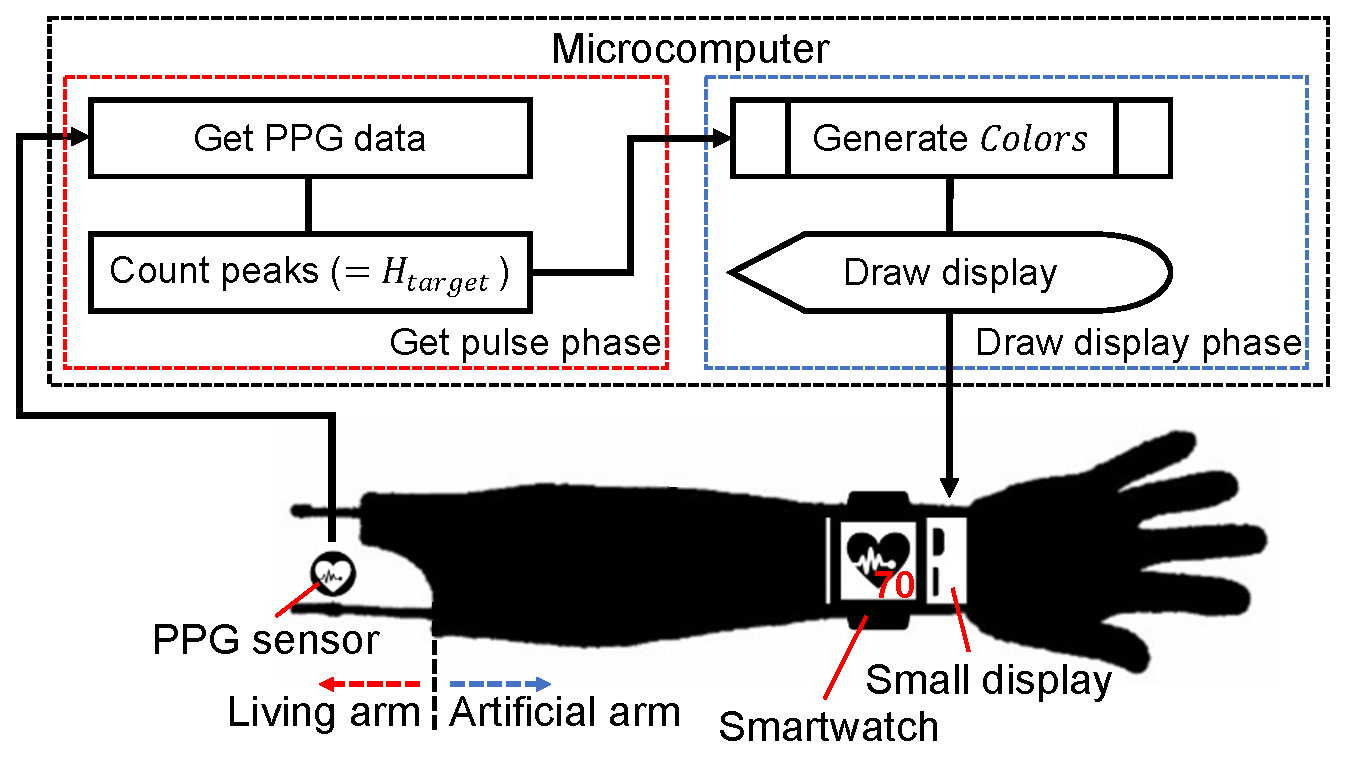
\includegraphics[width=1\linewidth]{figures/method.eps}
  \caption{Process flow of the proposed method.}
  \label{fig:method}
\end{figure}


% 3.2
\section{Target Heart Rate Calculation}
I denote the target heart, which is determined from the wearer's heart rate, as $H_{target}$. It is computed from two thresholds, $Threshold_{value}$ and $Threshold_{time}$, by using the PPG sensor, which constantly measures data. By using this data, the system records the times of pulse peak occurrences. A peak is detected when the PPG data measured in real time exceeds $Threshold_{value}$, but not until more than $Threshold_{time}$ time has passed since the last peak occurred. In this work, $Threshold_{value}$ and $Threshold_{time}$ were heuristically set to 700 and 0.3, respectively; in practice, however, they should be adjusted according to the environment in which the system is used. When a peak is detected, the time difference from the previous peak occurrence time is calculated. Here, the time difference refers to the RR interval, denoted as $RR$ [s], which is the time between one ventricular activation and the next. The number of times the ventricles contract in one minute is the heart rate in beats per minute (bpm). Therefore, if the RR interval is known, the heart rate $H_{target}$ can be calculated by the following equation:
\begin{equation}
  \label{eqn:target}
  H_{target} = int(60 / RR).
\end{equation}
The system continuously updates this value.\par

$H_{target}$ can also be set manually if the user wants the smartwatch to measure a specific heart rate. Figure \ref{fig:system} shows a system implementation in which the target heart rate is manually set from a control application and the heart rate is input to the smartwatch on an artificial arm.

\begin{figure}[!t]
  \centering
  \includegraphics[width=1\linewidth]{figures/system.eps}
  \caption{System implementation in which the target heart rate is manually set from a control application and the heart rate is input to the smartwatch on an artificial arm.}
  \label{fig:system}
\end{figure}


% 3.3
\section{Display Control}
Next, the display's brightness is controlled so that the heart rate measured by the smartwatch matches $H_{target}$. An array, denoted as $Colors$, is prepared in advance to store the required brightness for the smartwatch to detect a single pulse peak.\par

PPG sensors use LEDs to irradiate infrared, red, or green light onto the skin and measure pulse data from changes in the light reflected from the blood vessels. Because blood flow increases with the timing of the pulse, the blood vessels absorb more light, and the reflected light becomes dimmer. Because black absorbs more light than white, as the display is rendered blacker, the light emitted from the smartwatch and reflected by the display becomes darker.\par

Hence, the proposed method draws the values in $Colors$ on the display one by one during each drawing interval $T$ [s]. I set $T$ for each value in $Colors$ as follows, so that $Colors$ is applied $H_{target}$ times in one minute:
\begin{equation}
  \label{eqn:wait}
  T = 60 / \{len(Colors) * H_{target}\},
\end{equation}
where $len(Colors)$ is the data length of $Colors$.


% 3.4
\section{Pulse Data Measurement}
Finally, in the proposed method, pulse data is measured by the smartwatch worn over the blinking display. Such pulse data measured by a PPG sensor on a smartwatch can be used in various applications. However, the performance of the PPG sensor and the algorithm for measuring pulse data vary among different smartwatch models and are not publicly accessible. Accordingly, I manually set the target heart rate in my evaluation experiment described below.
